\apendice{Plan de Proyecto Software}

\section{Introducción}
En cualquier proyecto de este tipo es relevante incluir cierta información sobre la planificación, viabilidad y análisis de costes en el desarrollo del mismo con la finalidad de conseguir una visión de cómo ha ido evolucionando el proyecto y los ciclos de trabajo que se han llevado a cabo.

He de señalar que en la última tercera parte de los sprints, no siempre he contado con una línea de datos con la que poder replicar datos en GitHub, por lo que se han generado menos commits de los que se hubiera hecho si hubiera contado con medios a mi alcance. En cualquier caso, se ha intentado maximizar el número de puntos de salvado para que quedase constancia de la evolución del proyecto. Además, al redactar el proyecto en \LaTeX{} desde la plataforma de Overleaf no refleja el tiempo real invertido puesto que no se realizan cambios en el repositorio de forma automática, hasta que compilo, descargo y actualizo el repositorio manualmente.

En el primer apartado trataremos la~\textbf{planificación temporal}, donde podremos ver como han evolucionado los tiempos de trabajo durante las semanas en las que se ha trabajado en el proyecto. En el segundo apartado se reflejará un \textbf{estudio de viabilidad} sobre el proyecto, que a su vez incluye dos partes, la parte económica y la parte legal.

\section{Planificación temporal}
Al comenzar el proyecto se determinó que se utilizaría una metodología ágil para hacer el desarrollo del proyecto pero esta decisión ha terminado siendo un hándicap producido por la falta de documentación y la dudosa credibilidad de muchas páginas web y documentación que he encontrado, y se ha traducido en una gran inversión en tiempo.

Ante todo, se ha intentado seguir un mínimo de pautas~\textbf{Scrum}~\cite{manual:Scrum} pese a no existir un grupo de trabajo real con unas tareas diarias y roles definidos:
\begin{itemize}
    \item Las tareas fueron siempre semanales en forma de <<sprints>>.
    \item Al finalizar el sprint se hace la entrega del trabajo elaborado en la semana y se determinan las próximas tareas.
    \item Tras determinar las tareas se definen los <<milestones>> y los <<issues>>.
    \item Para hacer el seguimiento de las tareas se ha utilizado en tablero~\textbf{Kanban} de~\textbf{ZenHub}.
    \item Tras finalizar el sprint se puede comprobar el trabajo mediante los~\textit{gráficos burndown}.
\end{itemize}

Las reuniones de trabajo han sido consensuadas y planificadas para realizarlas los jueves de cada semana, con el siguiente resultado:

\begin{figure}
    \centering
    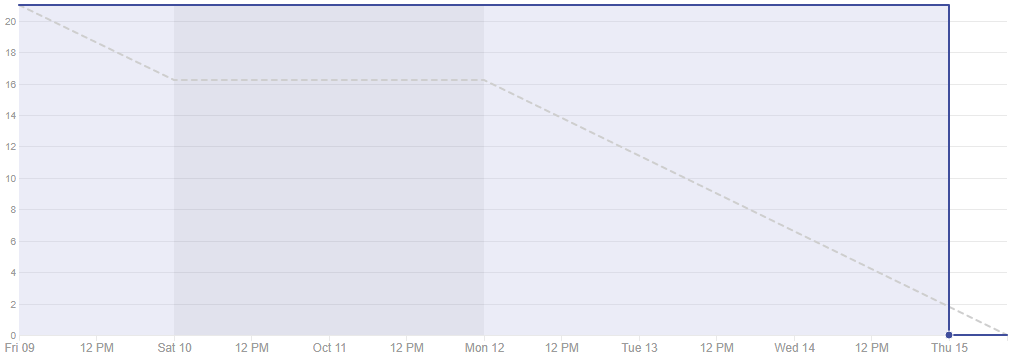
\includegraphics[width=0.9\textwidth]{img/BurnDown/1.PNG}
    \caption{Gráfico Burndown sprint1. } \label{BD1}
    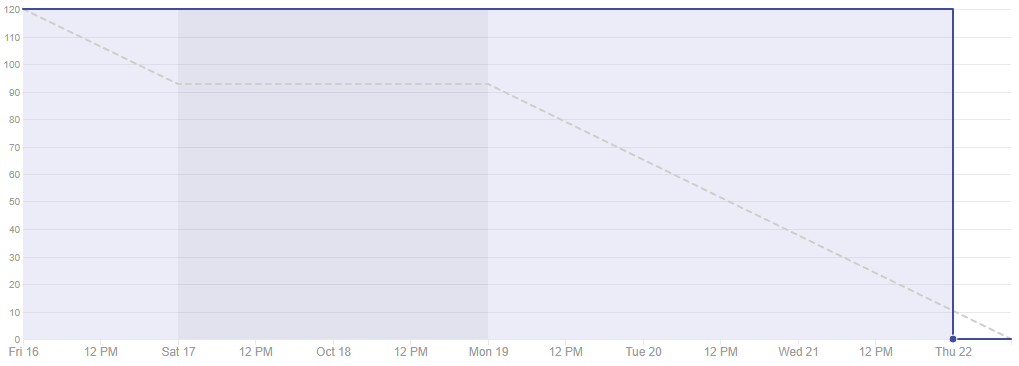
\includegraphics[width=0.9\textwidth]{img/BurnDown/2.PNG}
    \caption{Gráfico Burndown sprint2. } \label{BD2}
\end{figure}

\subsection{Sprint 00 - 01/10/2020 - 08/10/2020}
En la primera reunión nos reunimos Álvar Arnaiz González y yo. En ella hice la propuesta de temática del TFG y, además expuse diferentes ideas y enfoques sobre el proyecto en la que se determinó a grandes rasgos la posible viabilidad del proyecto.
Los objetivos de este <<sprint>> introductorio fueron la búsqueda de repositorios y otros proyectos para tomar ideas o si era posible hacer algún fork. También, el estudio la estructura del proyecto y herramientas software e interfaces a utilizar.

\subsection{Sprint 01 - 09/10/2020 - 15/10/2020}
Tras determinar el enfoque final de proyecto, se consensuó que los objetivos de este sprint fueron la búsqueda de información relevante, otros proyectos y recursos que puedan servir de utilidad como pueden ser APIS. Se buscaron algunas páginas web para realizar pruebas de extracción de datos con <<web scraping>>~\footnote{Se trata brevemente en el punto 4 de la memoria} y se descompusieron las tareas en unidades pequeñas de trabajo para poder afrontarlas durante sprints.

En este sprint también generé el repositorio en GitHub para poder trabajar contra él y podemos ver las líneas de código utilizadas en el \href{https://github.com/davidelinformatico/TFG/issues/1}{primer \textit{issue}}.

\begin{figure}
    \centering
    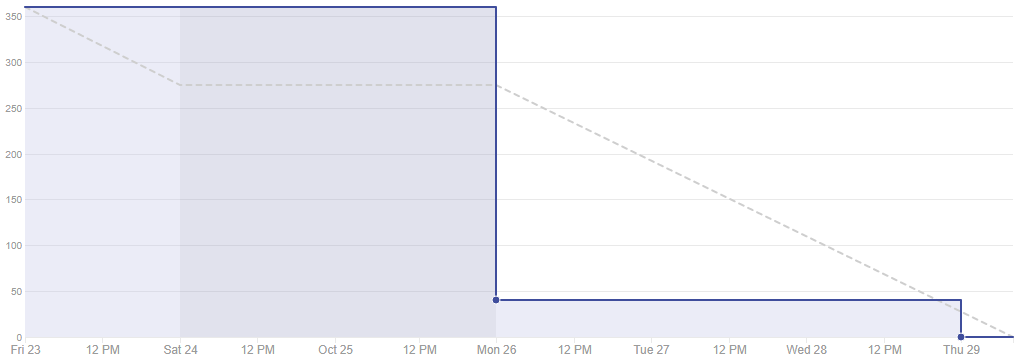
\includegraphics[width=0.9\textwidth]{img/BurnDown/3.PNG}
    \caption{Gráfico Burndown sprint3. } \label{BD3}
    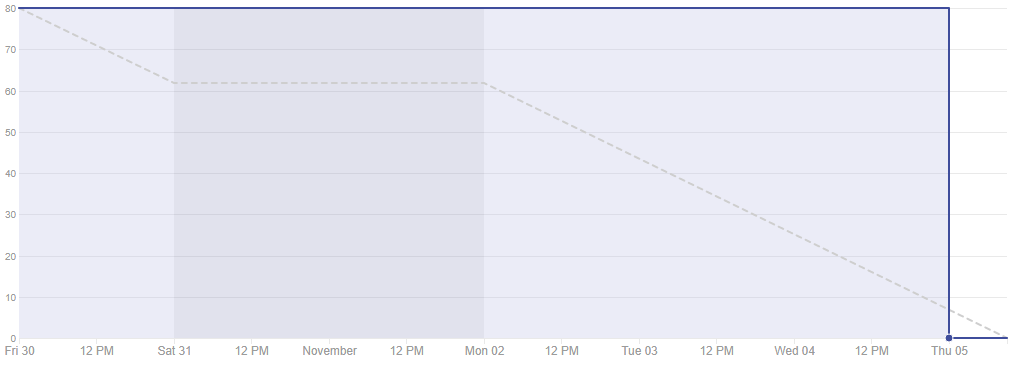
\includegraphics[width=0.9\textwidth]{img/BurnDown/4.PNG}
    \caption{Gráfico Burndown sprint4. } \label{BD4}
\end{figure}

\subsection{Sprint 02 - 16/10/2020 - 22/10/2020}
Los objetivos de este sprint fueron el buscar repositorios, APIS, servicios y tecnologías con las que darle forma al proyecto. Se decidió generar algún tipo de aplicación desde la que poder controlar la instalación haciéndola más amigable y con mejor capacidad de interacción. Se investigan opciones.

\item En el~\href{https://github.com/davidelinformatico/TFG/issues/2}{issue 2} se hizo una búsqueda por la web para buscar repositorios y proyectos sobre domótica
\item En el~\href{https://github.com/davidelinformatico/TFG/issues/3}{issue 3} buscamos algunas APIS para orientar el proyecto hacia el uso de APIS destinadas a ofrecer información que pueda servirnos y se realizaron algunas pruebas.
\item En el~\href{https://github.com/davidelinformatico/TFG/issues/4}{issue 4} se realizó un pequeño estudio de las tecnologías que podríamos utilizar, desde el procesador de textos, que finalmente se utilizó~\LaTeX{}, como la revisión de las normativas electrotécnicas que debía seguir en el proyecto y también se determinó la utilización de Telegram para interactuar con el Sistema Domótico.


\subsection{Sprint 03 - 23/10/2020 - 29/10/2020}
Los objetivos de este sprint fueron determinar los componentes hardware necesarios para completar el proyecto y se realiza la compra de material.
En todos los <<issues>> del <<\href{https://github.com/davidelinformatico/TFG/milestone/3?closed=1}{milestone 3}>> podemos ver múltiples enlaces, comparativas, justificaciones e imágenes en las que se ha basado toda la instalación física posterior.

\subsection{Sprint 04 - 30/10/2020 - 05/10/2020}
Se incorpora D.Alejandro Merino Gómez al que se le presenta el proyecto y se le concede acceso a los repositorios para que pueda co-tutorizar el proyecto.

Los objetivos de este <<milestone>> fueron todos de la parte física de la instalación:
\item Podemos ver en el \href{https://github.com/davidelinformatico/TFG/issues/15}{issue 15} que finalicé la tirada de cable junto a un diagrama explicativo del funcionamiento de un pulsador de 3 posiciones (Posición 1, Reposo y Posición 2. Teniendo en cuenta que las dos posiciones que dan continuidad al circuito tienen invertida la polaridad).
\item También vemos en el \href{https://github.com/davidelinformatico/TFG/issues/16}{issue 16} la presentación de la Raspberry Pi que utilizaremos, los conectores del tipo JST-XH que se han utilizado en el crimpado de los cables electrónicos, los cables finalizados con sus conectores y la disposición final de la Raspberry Pi en su ubicación final de la instalación.

\begin{figure}
    \centering
    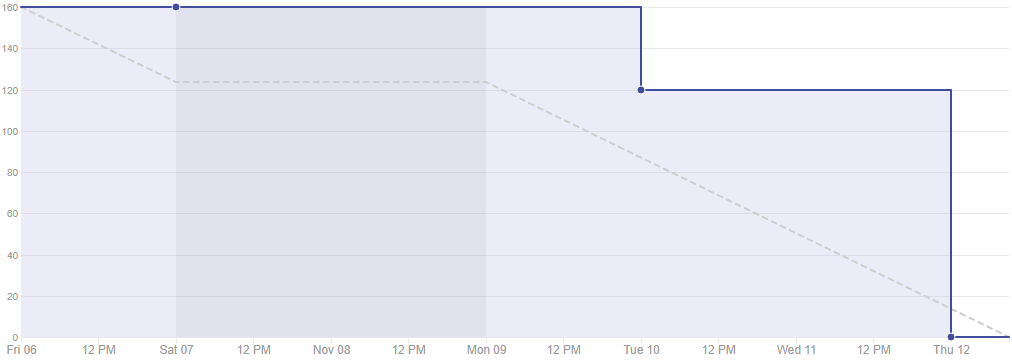
\includegraphics[width=0.9\textwidth]{img/BurnDown/5.PNG}
    \caption{Gráfico Burndown sprint5. } \label{BD5}
    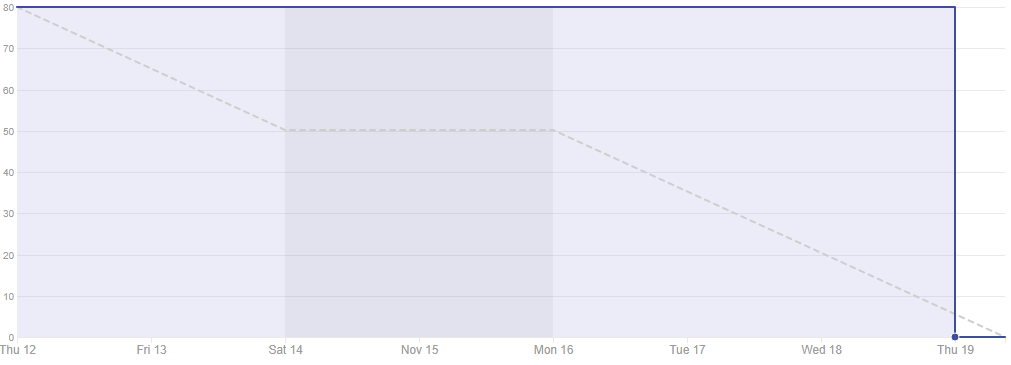
\includegraphics[width=0.9\textwidth]{img/BurnDown/6.PNG}
    \caption{Gráfico Burndown sprint6. } \label{BD6}
\end{figure}

\subsection{Sprint 05 - 06/11/2020 - 12/11/2020}
Se repasan los cambios propuestos y se incluyen otros nuevos sobre la parte física de la instalación. Se hace el seguimiento de la instalación y se comentan las fotos y el estado de la instalación.
Los objetivos de este sprint son todos aquellos que sean necesarios para la adecuación del software básico para comenzar el proyecto como la actualización del sistema operativo o instalación de software adicional. Además se deben valorar opciones para controlar los GPIO.

\item Vemos en los issues \href{https://github.com/davidelinformatico/TFG/issues/21}{21} y \href{https://github.com/davidelinformatico/TFG/issues/19}{19} las configuraciones básicas realizadas a nuestro Raspbian. Para explicar este proceso grabé dos vídeos, titulados \href{https://youtu.be/B8E6q1fLp7Q}{Primeros Pasos Raspberry Pi} y \href{https://youtu.be/Vz38sGYpcYQ}{Actualización de Raspberry Pi y configuración básica}, respectivamente.

\subsection{Sprint 06 - 13/11/2020 - 19/11/2020}
Se revisan los puntos anteriores y se compone un tablero de pruebas de forma que se puede controlar el encendido de una bombilla desde nuestra Raspberry Pi. También se graba un vídeo explicativo y se diseñan unos diagramas explicativos.

Podemos ver en el \href{https://github.com/davidelinformatico/TFG/issues/22}{issue 22} que se presenta un diagrama con la lista de los componentes que vamos a utilizar en el tablero de pruebas y un diagrama de como se compondrá el tablero. En este issue también grabé un vídeo para explicar el tablero de pruebas y decidí utilizar un efecto más conservador de cara al final del proyecto.

En el \href{https://github.com/davidelinformatico/TFG/issues/23}{issue 23} he explicado como se controlan los GPIO de nuestra Raspberry Pi desde su distribución Linux~\footnote{Raspbery pi (Raspbian OS).} desde Bash y desde Python.

\begin{figure}
    \centering
    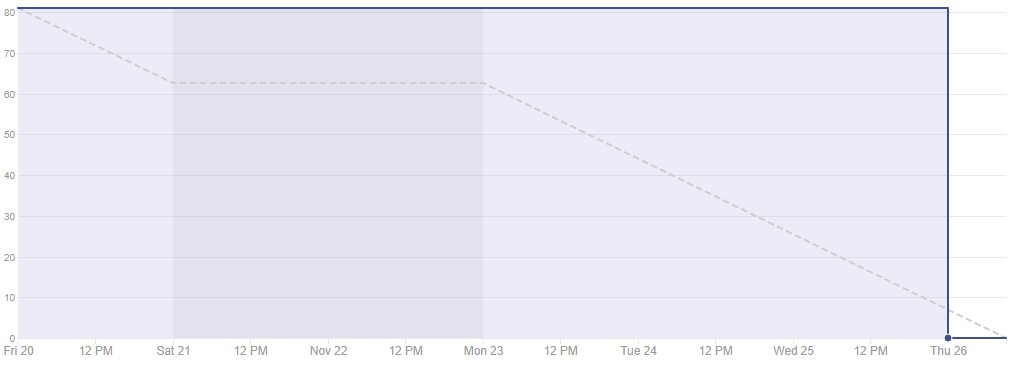
\includegraphics[width=0.9\textwidth]{img/BurnDown/7.PNG}
    \caption{Gráfico Burndown sprint7. } \label{BD5}
    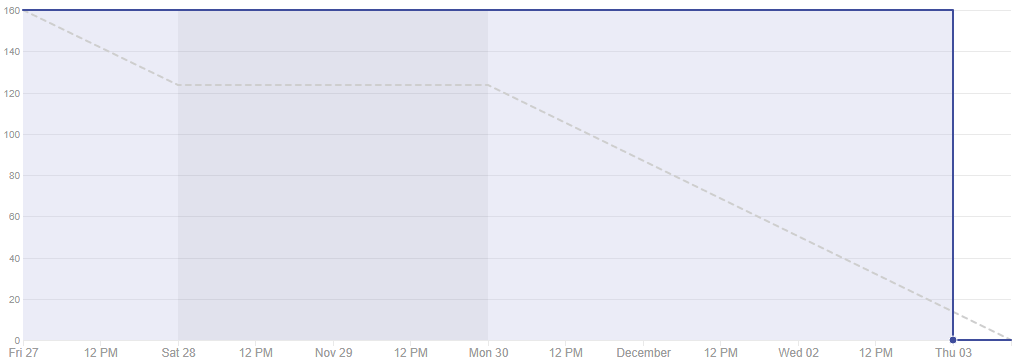
\includegraphics[width=0.9\textwidth]{img/BurnDown/8.PNG}
    \caption{Gráfico Burndown sprint8. } \label{BD6}
\end{figure}

\subsection{Sprint 07 - 20/11/2020 - 26/11/2020}
Se realiza una investigación sobre como se puede implantar el bot en nuestro proyecto, se realiza el primer código de pruebas y se presentan las primeras pruebas con el bot. Podemos ver en el \href{https://github.com/davidelinformatico/TFG/issues/13}{issue 13} un resumen de las pruebas que estuve realizando con los diferentes teclados de que dispone Telegram.

también, se proponen correcciones en la redacción.

\subsection{Sprint 08 - 27/11/2020 - 03/12/2020}
En el \href{https://github.com/davidelinformatico/TFG/milestone/8?closed=1}{milestone 8}, podemos ver que se incluyen varios issues:

\begin{itemize}
    \item Creación de scripts Bash para controlar el conjunto del Sistema Domótico inteligente.
    \item Obtención de los datos de geolocalización y cálculo de temperaturas.
    \item Generación del nuevo Cron tras integrar los scripts existentes.
\end{itemize}

De esta manera, se genera la primera automatización completa de la parte automática del proyecto utilizando CRON y lo pasamos del entorno de pruebas a un entorno de producción en fase experimental. En este momento únicamente tenemos control sobre la máquina de forma física o por VNC.
Por último, se presentan las primeras funcionalidades del bot, se proponen cambios y mejoras.


\subsection{Sprint 09 - 04/12/2020 - 10/12/2020}
En el \href{https://github.com/davidelinformatico/TFG/milestone/9?closed=1}{milestone 9} se proponen revisan las funcionalidades del Bot~\cite{misc:TelegramApi} de Telegram~\cite{misc:TelegramApp} que utilizaremos, se proponen cambios y mejoras en el código preexistente en fase de pruebas.

Finalmente se integra un bot de Telegram completamente funcional desde el que podremos lanzar órdenes a nuestro sistema domótico con los scripts existentes.

\begin{figure}
    \centering
    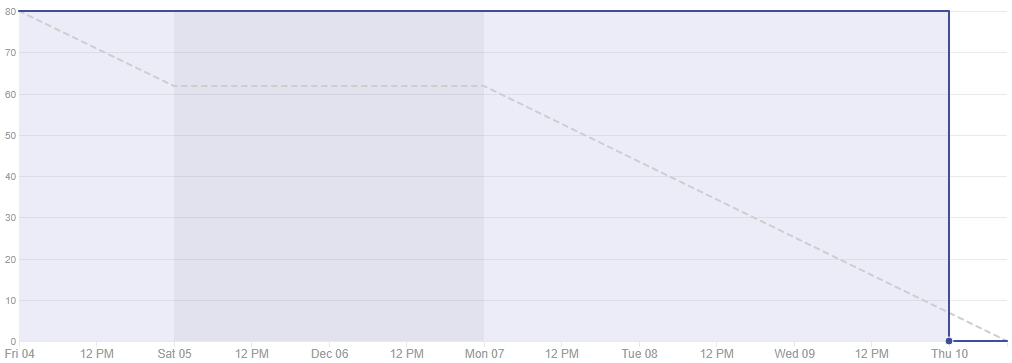
\includegraphics[width=0.9\textwidth]{img/BurnDown/9.PNG}
    \caption{Gráfico Burndown sprint9. } \label{BD9}
    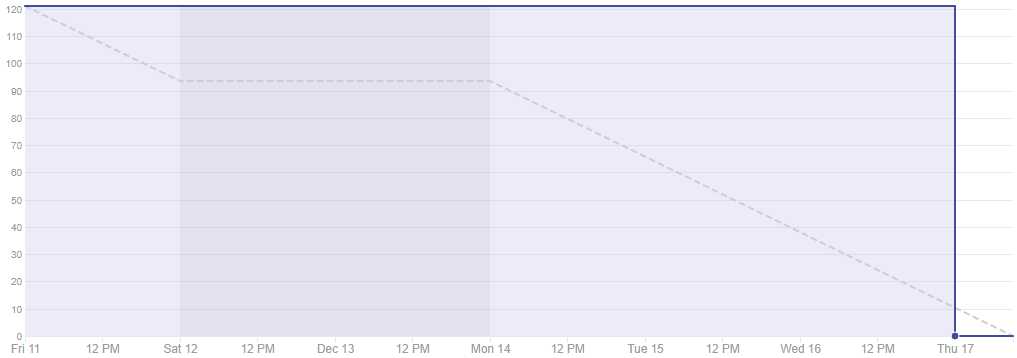
\includegraphics[width=0.9\textwidth]{img/BurnDown/10.PNG}
    \caption{Gráfico Burndown sprint10. } \label{BD10}
\end{figure}

\subsection{Sprint 10 - 11/12/2020 - 17/12/2020}
En el \href{https://github.com/davidelinformatico/TFG/milestone/10?closed=1}{milestone 10} se ha aprovechado para optimizar las rutas de los archivos a los que se invoca desde el código en ejecución y se han modificado algunas salidas para que tengan un aspecto visual más atractivo, incluyendo tablas, emoticonos desde Unicode~\cite{misc:UnicodeWikipedia}.

Se comprueban las funcionalidades proponiendo cambios funcionales y de estilos de forma que se pueda interactuar contra el bot y se muestren los mensajes en un formato más atractivo. También se propone unificar las rutas de trabajo de los diferentes scripts.


\subsection{Sprint 11 - 18/12/2020 - 24/12/2020}
Se propone dividir el código por funcionalidades (obtención de información de la web, y por otro lado, modificación de archivos del sistema y se proponen cambios en la redacción a implementar en el sprint 12.

Finalmente, se ha conseguido generadr la división del código en 3 archivos principales:
\begin{enumerate}
    \item Toma de datos de la web y guardado en json.
    \item Lectura de parámetros personalizados.
    \item Grabado de CRON conforme a esas preferencias.
\end{enumerate}

De esta manera conseguimos minimizar las comunicaciones con el exterior y poder relanzar el código separado por funcionalidad lógica de forma que podamos relanzarlo de forma aislada en caso de necesitarlo. Un ejemplo puede ser cuando se modifica la hora de subida de las persianas, el módulo de generación de CRON leería el archivo de parámetros personalizados y generaría la configuración a partir de éstos.

\begin{figure}
    \centering
    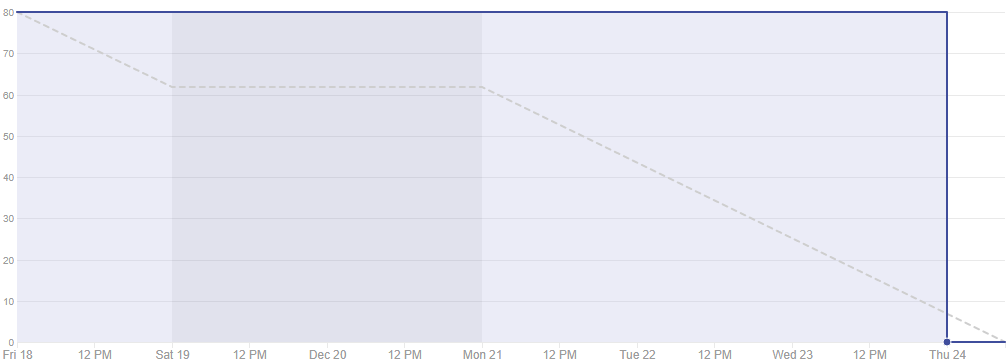
\includegraphics[width=0.9\textwidth]{img/BurnDown/11.PNG}
    \caption{Gráfico Burndown sprint11. } \label{BD11}
\end{figure}

\subsection{Sprint 12 - 30/12/2020 - 06/01/2021}
Se finaliza la redacción de la memoria, antes de la revisión final del texto, y se comienza con los anexos. Además se produce depurado del código y se utiliza SonarCloud.

\subsection{Sprint 13 - 07/01/2020 - 13/01/2020}
Redacción del proyecto del TFG y grabado de vídeos.

\subsection{Sprint 14 - 14/01/2020 - 20/01/2020}
Edición de vídeos y entrega.


\section{Estudio de viabilidad}

\subsection{Viabilidad económica}

\subsection{Viabilidad legal}


